\documentclass[numbers=noenddot, openany]{thesis}

% hier namen etc. einsetzen
\fullname{Lukas Hennig\\Felix Rottler\\Natalie Spister}
\headline{Advanced Mobile Business Applications\\Dokumentation}
\jahr{2018}
\gutachterA{Marc Schickler}
\typ{Anwendungsfach }
\fakultaet{Ingenieurwissenschaften, Informatik und \\Psychologie}
\institut{Institut für Datenbanken und Informationssysteme}

\hypersetup{%
	pdftitle=\pdfescapestring{\thetitel},
	pdfauthor={\thefullname},
 	pdfsubject={\thetyp},
}


\usepackage{graphicx}
\usepackage{caption}
\usepackage{subcaption}
\usepackage{float}


% trennungsregeln
\hyphenation{Sil-ben-trenn-ung}

\begin{document}
\frontmatter
\maketitle
% impressum
\impressum

% ab hier zeilenabstand 1,4 fach 10pt/14pt
\setstretch{1.4}

\section*{Kurzfassung}
Im Rahmen der Veranstaltung Advanced Mobile Application Engineering 

Die Kurzfassung (engl. Abstract) einer Abschlussarbeit enthält zwei Blöcke. Der
erste Block enthält eine  kurze Hinführung/Motivation zum Thema sowie einer
anschließenden Beschreibung der Problemstellung (ca. 5-8 Sätze). Der zweite
Block der Kursfassung gibt die Zielsetzung bzw. den Beitrag der Abschlussarbeit
wieder (ebenfalls ca. 5-8 Sätze).

===========================================

ChangeLog:

2015-10-12: Hacks für Literaturverzeichnis eingebaut. Kommentare in der BibTex
Datei beachten!

2015-07-21: Fakultätname angepasst (+ Psychologie)




% inhaltsverzeichnis einfügen
\tableofcontents

\mainmatter
% hier kommen die kapitel der arbeit
% % %
%
%	- Einleitung- 
%
%	Ziel:	Gib eine schöne Einleitung mit Motivation, Problemstellung, Zielsetzung und Struktur der Arbeit
%
%	Status: alpha
%
% % %
\chapter{Einleitung}
\label{cha:einleitung}
Hier kommt die Einleitung mit Motivation hin.

% Abschnitt: Problemstellung
\section{Problemstellung}
\label{sec:einleitung:problemstellung}
Beschreibe in diesem Abschnitt die Problemstellung der Arbeit!

% Abschnitt: Zielsetzung
\section{Zielsetzung}
\label{sec:einleitung:zielsetzung}
Beschreibe in diesem Abschnitt die Zielsetzung der Arbeit!

% Abschnitt: Struktur der Arbeit
\section{Struktur der Arbeit}
\label{sec:einleitung:struktur}
Beschreibe in diesem Abschnitt die Struktur der Arbeit!

\chapter{Grundlagen}
\label{cha:grundlagen}
In diesem Abschnitt werden kurz einige Grundlagen, die für das Spiel wichtig sind, erklärt. 

%Abschnitt: Jump 'n' Run
\section{Jump 'n' Run (Platformer)}
\label{sec:grundlagen:jumpnrun}
Die Anwendung soll das vorhandene Spielprinzip des Jump 'n' Runs übernehmen und eigene Ideen einfließen lassen. Wie der Name schon suggeriert zeichnet sich ein Jump 'n' Run - Spiel dadurch aus, dass die Spielfigur durch \textit{springen} und \textit{laufen} Hindernisse überwinden und in den meisten Fällen ein Ziel erreichen muss. Zusätzlich kann dem Spieler die Möglichkeit gegeben werden zu \textit{schießen}, zu \textit{klettern} oder zu \textit{kämpfen}. \\
Das klassiche Jump 'n' Run ist in 2D und die Spielfigur läuft von links nach rechts, wobei der Fokus der Kamera stets auf der gesteuerten Spielfigur liegt. 


%Abschnitt: Multiplayer
\section{Multiplayer}
\label{sec:grundlagen:multiplayer}
Klassische Jump'n'Run Spiele wie Mario sind für Einzelspieler konzipiert, aber schon mit der ersten Playstation \cite{playstation} setzten sich Multiplayerspiele durch, zunächst waren aufgrund der begrenzten Controller nur zwei Spieler möglich. Kabellose Controller und der Durchbruch des Internets eröffneten jedoch die Möglichkeit einer nahezu unbegrenzten Anzahl von Spielern ein gemeinsames Spielerlebnis. \\
Um dies zu ermöglichen wird auf einer mobilen Platform eine Verbindung zu einem Server, also damit ein Server und eine bestehende Internetverbindung benötigt. Die Spiellogik selber wird über ein Netzwerk realisiert, ein Beispiel für solch ein Netzwerk sind die \textit{Google Play Services} \cite{googleplayservices} von Google. In Unity gibt es dafür das \textit{Photon Unity Networking}, welches in Kapitel \ref{subsec:realisierung:technologien:photon} genauer betrachtet wird.


% Abschnitt: Spielgrundlagen
\section{Spielablauf}
\label{sec:grundlagen:spielgrundlagen}
Abyss soll ein levelbasiertes Jump'n'Run Multiplayer Spiel werden. \newline
Ganz wie andere Platformer sollen die Spieler sich auf Plattformen in eine Richtung bewegen. Da das Spiel levelbasiert sein soll, ist das Ziel des Spielers das Ende eines jeden Levels zu erreichen und ins nächste Level zu gelangen. \\
Um Eintönigkeit beim Spiel zu vermeiden werden die Level mit unterschiedlichen Schwierigkeiten implementiert, dabei sollen nicht nur Spielitems wie z.B. Power-Ups zum Einsatz kommen, sondern auch bewegliche Objekte, die dem Spieler auch Schaden hinzufügen können. \\
Damit der Spieler sich möglichst gut im Spiel zurechtfindet wird die Steuerung minimal und möglichst einfach gehalten, so können auch Fehleingaben vermieden werden. Des Weiteren soll das Spiel nur im Multiplayermodus gespielt werden können, also werden immer zwei Spieler benötigt um das Spiel zu starten. 
% Steuerung Anfoderung

\chapter{Anforderungen}
\label{cha:anforderungen}
In diesem Kapitel werden die Anforderungen an das Spiel definiert. Dabei legen die funktionalen Anforderungen fest, wozu das Spiel imstande sein soll. Die nicht-funktionalen Anforderungen beschreiben, wie gut diese Anforderungen umgesetzt werden sollen.

% Abschnitt: Funktionale Anforderungen
\section{Funktionale Anforderungen}
\label{sec:grundlagen:funktionaleAnforderungen}
In Tabelle \ref{tab:grundlagen:funktionaleAnforderungen} werden die funktionalen Anforderungen an das Spiel und die jeweilige Priorisierung mit Werten von 1 (unwichtig) bis 5 (unabdingbar) formuliert.

\begin{center}
    \label{tab:grundlagen:funktionaleAnforderungen}
    \begin{tabular}{ c | l | c}
        Abkürzung & Anforderung & Priorität\\
        \hline
        FA01 & An- und Abmelden & 4 \\
        \hline
        FA02 & Spiel erstellen & 5 \\
        \hline
        FA03 & Spiel beitreten & 5 \\
        \hline
        FA04 & Multiplayer (2 Spieler) & 5 \\
        \hline
        FA05 & Animation der Spieler & 4 \\
        \hline
        FA06 & Verschiedene Level & 4 \\
        \hline
        FA07 & Verschiedene Level-Themen & 3 \\
        \hline
        FA08 & Verschiedene Spielobjekte & 4 \\
        \hline
        FA09 & Animation der Spielobjekte & 2 \\
        \hline
        FA10 & Simple Spielsteuerung & 5 \\
    \end{tabular}
    \captionof{table}{Funktionale Anforderungen} 
\end{center}

\textbf{FA01 An- und Abmelden}\\*
Der Nutzer kann sich im Spiel anmelden. Anschließend kann er das Spiel uneingeschränkt verwenden. Er bleibt so lange angemeldet bis er sich abmeldet.

\textbf{FA02 Spiel erstellen}\\*
Ein Spiel kann von jedem angemeldeten Nutzer erstellt werden. Dabei kann der Nutzer nur die Level verwenden, die er freigeschalten hat.

\textbf{FA03 Spiel beitreten}\\*
Jeder Nutzer kann jedem beliebigen Spiel beitreten unabhängig davon welche Level der Nutzer selbst freigeschalten hat.

\textbf{FA04 Multiplayer}\\*
Das Spiel soll ausschließlich von zwei Nutzern gespielt werden können. Die Nutzer sollen dabei den jeweiligen Mitspieler auf ihrem eigenen Gerät sehen können. Zudem soll teilweise ein kooperatives Spiel zwischen den Spielern erzwingbar sein.

\textbf{FA05 Animation der Spieler}\\*
Die verschiedenen Möglichkeiten der Steuerung eines Spielers sollen mit Animationen unterlegt werden. 

\textbf{FA06 Verschiedene Level}\\*
Es soll mehr als ein Level geben. Der Nutzer hat anfangs nur die Möglichkeit das erste Level zu spielen. Erst nach Abschluss eines Levels wird das nächste freigeschalten.

\textbf{FA07 Verschiedene Level-Themen}\\*
Die Level sollen sich im Design voneinander unterscheiden. Die Spielerfiguren und Spielobjekte bleiben dabei die gleichen im Aussehen und in ihrer Funktion.

\textbf{FA08 Verschiedene Spielobjekte}\\*
Durch verschiedene Spielobjekte innherhalb des Spiels wird das Spiel abwechslungsreich und komplex. Jedes dieser Spielobjekte hat dabei einen unterschiedlichen Effekt.

\textbf{FA09 Animation der Spielobjekte}\\*
Die Spielobjekte sollen durch Animationen als solche hervorgehoben werden. Dabei können sie bei Aktivierung verschiedene Effekte/Animationen/Geräusche machen, die den Zweck des Spielobjekts entprechen.

\textbf{FA10 Simple Spielsteuerung}\\*
Das Spiel soll möglichst einfach gesteuert werden können, d.h. auch das Eingaben, die möglicherweise falsch interpretiert werden können (Wischen in verschiedene Richtungen oder langes Drücken), sollen möglichst vermieden werden.


% Abschnitt: Nicht-Funktionale Anforderungen
\section{Nicht-Funktionale Anforderungen}
\label{sec:grundlagen:nichtFunktionaleAnforderungen}
Die in Kapitel \ref{sec:grundlagen:funktionaleAnforderungen} beschriebenen funktionale Anforderungen bestimmen die Funktionen und Umfang des Spiels. In der Tabelle \ref{tab:grundlagen:nichtFunktionaleAnforderungen} werden nun die nichtfunktionalen Anforderungen dargelegt, die die Qualität der Umsetzung festlegen.

\begin{center}
    \label{tab:grundlagen:nichtFunktionaleAnforderungen}
    \begin{tabular}{ c | l | c}
        Abkürzung & Anforderung & Priorität\\
        \hline
        NFA01 & Zuverlässigkeit & 5 \\
        \hline
        NFA02 & Aussehen und Handhabung & 5 \\
        \hline
        NFA03 & Benutzbarkeit & 4 \\
        \hline
        NFA04 & Funktionalität & 5 \\
        \hline
        NFA05 & Effizienz & 3 \\
    \end{tabular}
    \captionof{table}{Nichtfunktionale Anforderungen} 
\end{center}

\textbf{NFA01 Zuverlässigkeit}\\*
Das Spiel ist konsistent in der Ausführung. Es bricht nicht unerwartet ab und jedes Level kann von beiden Spielern beendet werden.

\textbf{NFA02 Aussehen und Handhabung}\\*
Das Spiel hinterlässt einen einen guten optischen Eindruck und besitzt eine uintuitive Steuerung.

\textbf{NFA03 Benutzbarkeit}\\*
Der Ablauf des Spiels ist leicht ersichtlich, sowohl im Menü als auch in den jeweiligen Level.

\textbf{NFA04 Funktionalität}\\*
Die in Kapitel \ref{sec:grundlagen:funktionaleAnforderungen} vorgestellten Anforderungen werden abhängig von ihrer Priorisierung erfolgreich umgesetzt.

\textbf{NFA05 Effizienz}\\*
Das Spiel soll auf dem eigenen als auch auf dem Gerät des Mitspielers flüssig laufen. 




\chapter{Konzeption \& Entwurf}
\label{cha:konzeption}
In diesem Kapitel wird das anfängliche Spielkonzept mit Hilfe von Mock-Ups visualisiert und evaluiert. Anschließend wird in Kapitel \ref{sec:konzeption:konzept} das umgesetzte Spielkonzept vorgestellt.

\section{Mock-Ups}
\label{sec:konzeption:prototyping:mockups}
Die ursprüngliche Idee des Spiels war ein Spielverlauf von oben nach unten, wodurch die beiden Spieler einen Abgrund (\textit{Abyss}) hinabspringen müssen, um einen Endgegner zu bekämpfen. Dabei springen beide Spieler durchgehend und um mit der Device-Motion die Richtung zu ändern (ähnlich zu \href{https://play.google.com/store/apps/details?id=com.lima.doodlejump&hl=de}{\textit{Doodle Jump}}). Jedoch sind durch dieses Leveldesign die Möglichkeiten der Levelgestaltung, als auch die Bewegungsfreiheit der Spieler stark eingeschränkt.
\begin{figure}[H]
    \begin{center}
      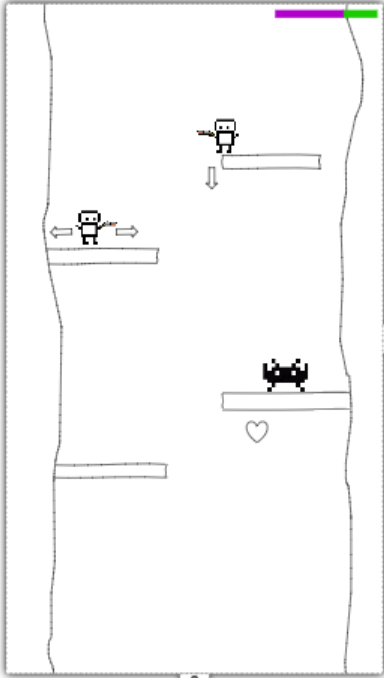
\includegraphics[width=.22\linewidth]{img/konzeption/Jump}
      \caption{Steuerung}
      \label{fig:konzeption:prototyping:jump}
    \end{center}
\end{figure}


Zusätzlich sollten Waffen in dem Spiel eingesetzt werden können, jedoch sind die Steuerungsmöglichkeiten an einem Smartphone mit den Möglichkeiten zu springen, schießen und bewegen des Spielers stark eingeschränkt und fehleranfällig.

\begin{figure}[H]
    \begin{center}
      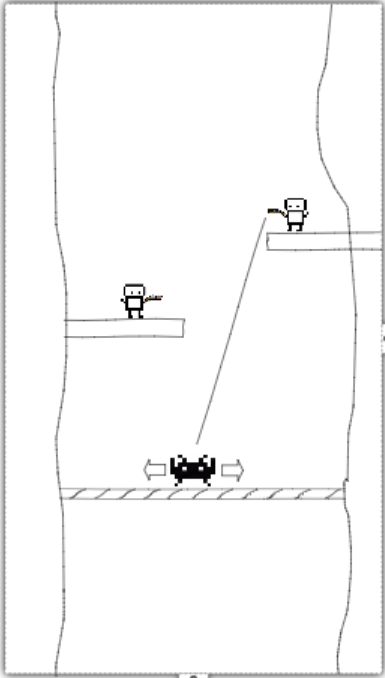
\includegraphics[width=.22\linewidth]{img/konzepFtion/Fight}
      \caption{Waffen}
      \label{fig:konzeption:prototyping:fight}
    \end{center}
\end{figure}


Zur Beendigung des Levels müssen beide Spieler das Ende erreichen um anschließend einen Endgegner zu besiegen. Wie in Kapitel \ref{sec:implementierung:probleme} erklärt, ist das designen von Assets anspruchsvoll und zeitaufwendig.
\begin{figure}[H]
    \begin{center}
      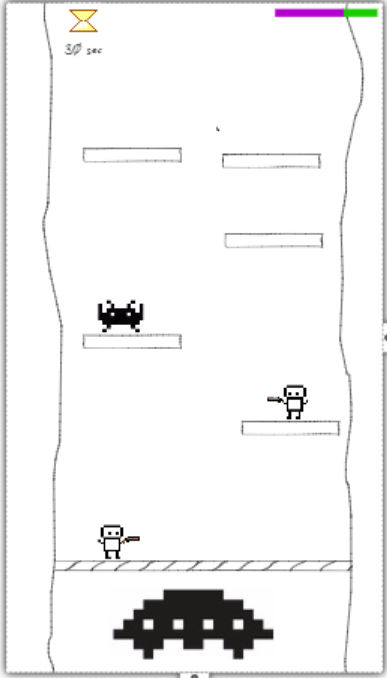
\includegraphics[width=.22\linewidth]{img/konzeption/EndBoss}
      \caption{Endboss}
      \label{fig:konzeption:prototyping:endboss}
    \end{center}
\end{figure}

\section{Spielkonzept}
\label{sec:konzeption:konzept}
In diesem Kapitel werden Spieleigenschaften, der Aufbau der Level und der Funktionsumfang der verschiedenen Spielobjekte erläutert. Die Ansicht der Spiels ist zweidimensional, daher werden die Level stets von der Seite dargestellt.

\subsection{Level}
\label{sec:konzeption:konzept:level}
 Die jeweiligen Level des Spiels beschäftigen sich mit einem eigenen Thema (mit eigenem Licht, Musik und Umfeld). Um ein Zusammenspielen der Spieler zu erzwingen müssen beide Spieler das Level beenden. Erst wenn beide Spieler das Ziel erreichen, ist das Level beendet. Damit das Level beendet werden kann, müssen im Laufe des Spiels zwei Schlüssel eingesammelt, die es erst ermöglichen das Ziel in Form einer Truhe zu erreichen. Spieler können anfangs nur das erste Level spielen, erst nach Beendigung des Levels wird das darauffolgende Level freigeschalten und somit spielbar. 

\subsection{Spielobjekte}
\label{sec:konzeption:konzept:spielobjekte}
Um das Spiel für den Spieler attraktiver zu gestalten werden verschiedene Spielobjekte verwendet, die das Spiel interessanter und abwechslungsreicher gestalten sollen. Diese Spielobjekte können den Spieler einen Vorteil verschaffen (\textit{Power-Up}), Schaden zufügen (\textit{Gegner}) oder transportieren (\textit{Plattform}). Zusätzlich gibt es Spielobjekte, die das Passieren eines bestimmten Spielers verhindern (\textit{Barriere}) und somit einen Weg erzwingt, der sich von dem des anderen Spielers unterscheidet. Um entfernte oder abgeschnittene Spielbereiche zu erreichen und das Spiel somit komplexer zu gestalten werden \textit{Portale} verwendet, die den Spieler zu einem zugehörigen Portal transportieren. Wie bereits in Kapitel \ref{sec:konzeption:konzept:level} erwähnt existieren genau zwei \textit{Schlüssel}, die zum Beendigen des Levels benötigt werden. Das Ziel des Spiels hat die Form einer \textit{Truhe}, die von beiden Spielern erreicht werden muss.

\subsection{Spieler}
\label{sec:konzeption:konzept:spieler}
Da das Spiel für genau zwei Spieler ausgelegt ist, werden für die gleiche Spielfigur zwei verschiedene Farben verwendet um die Spieler darzustellen und zu unterscheiden. Die Handlungsmöglichkeiten der Spieler sind auf Laufen (nach rechts oder links) und Springen beschränkt. Spieler sind zusätzlich in der Lage Wall-Jumps (abspringen an einer Wand) zu vollziehen.

Kommt ein Spieler mit einem Hindernis in Kontakt verliert der jeweilige Spieler je nach Hindernis ein Teil seines Lebens. In Spielen wie \textit{Super Mario} stirbt der Spieler sofort nach Kontakt mit einem Hindernis. Sollte ein Spieler im Laufe eines Levels sterben, müssen beide Spieler das Level von vorne beginnen.

Um das Zusammenspielen in bestimmten Level zu erzwingen und um das Spiel um eine Feature zu erweitern, erhält der zurückbleibende Spieler schaden, falls der Abstand zwischen Ihm und dem Mitspieler zu groß wird.

\subsection{Steuerung}
\label{sec:konzeption:konzept:steuerung}
Um die Nutzung der Anwendung übersichtlich zu halten wird die Spielsteuerung möglichst simpel gestalten. Die Bewegung des Spielers von links nach rechts wird am Smartphone durch die Device-Motion ermöglicht (Neigung des Smartphones). Um die Touchgesten einfach zu halten, kann der Spieler mit einem Klick springen. Gleitet der Spieler eine Wand herunter, kann zu diesem Moment der Sprung verwendet werden, um von der Wand abzuspringen und so einen Wall-Jump zu vollziehen. 

Am Computer wird für die Steuerung die links bzw. rechts Taste verwendet. Zum Springen muss die Leertaste betätigt werden.


% Abschnitt: Layout
\section{Layout}
\label{sec:konzeption:layout}
Das Spiel soll bis zum Spielstart einen geregelten Ablauf haben. Die Spieler haben nach dem Spielstart die Möglichkeit sich mit ihrem Account anzumelden oder zu registrieren. Anschließend wird das Hauptmenü der Anwendung angezeigt. Dort hat man die Möglichkeit einen Raum zu erstellen oder einem bereits bestehenden Raum beizutreten. Erstellt ein Spieler einen Raum muss er noch das Level auswählen, das gespielt werden soll. Anschließend wartet der Spieler, der den Raum erstellt hat, auf den anderen Spieler und kann das Spiel im ausgewählten Level starten. Die Abbildung \ref{fig:konzeption:layout:menu} zeigt diesen Menu-Ablauf bis zum Starten des Spiels. Jeder Zustand repräsentiert dabei einen Screen der Anwendung. 

\begin{figure}[H]
    \begin{center}
      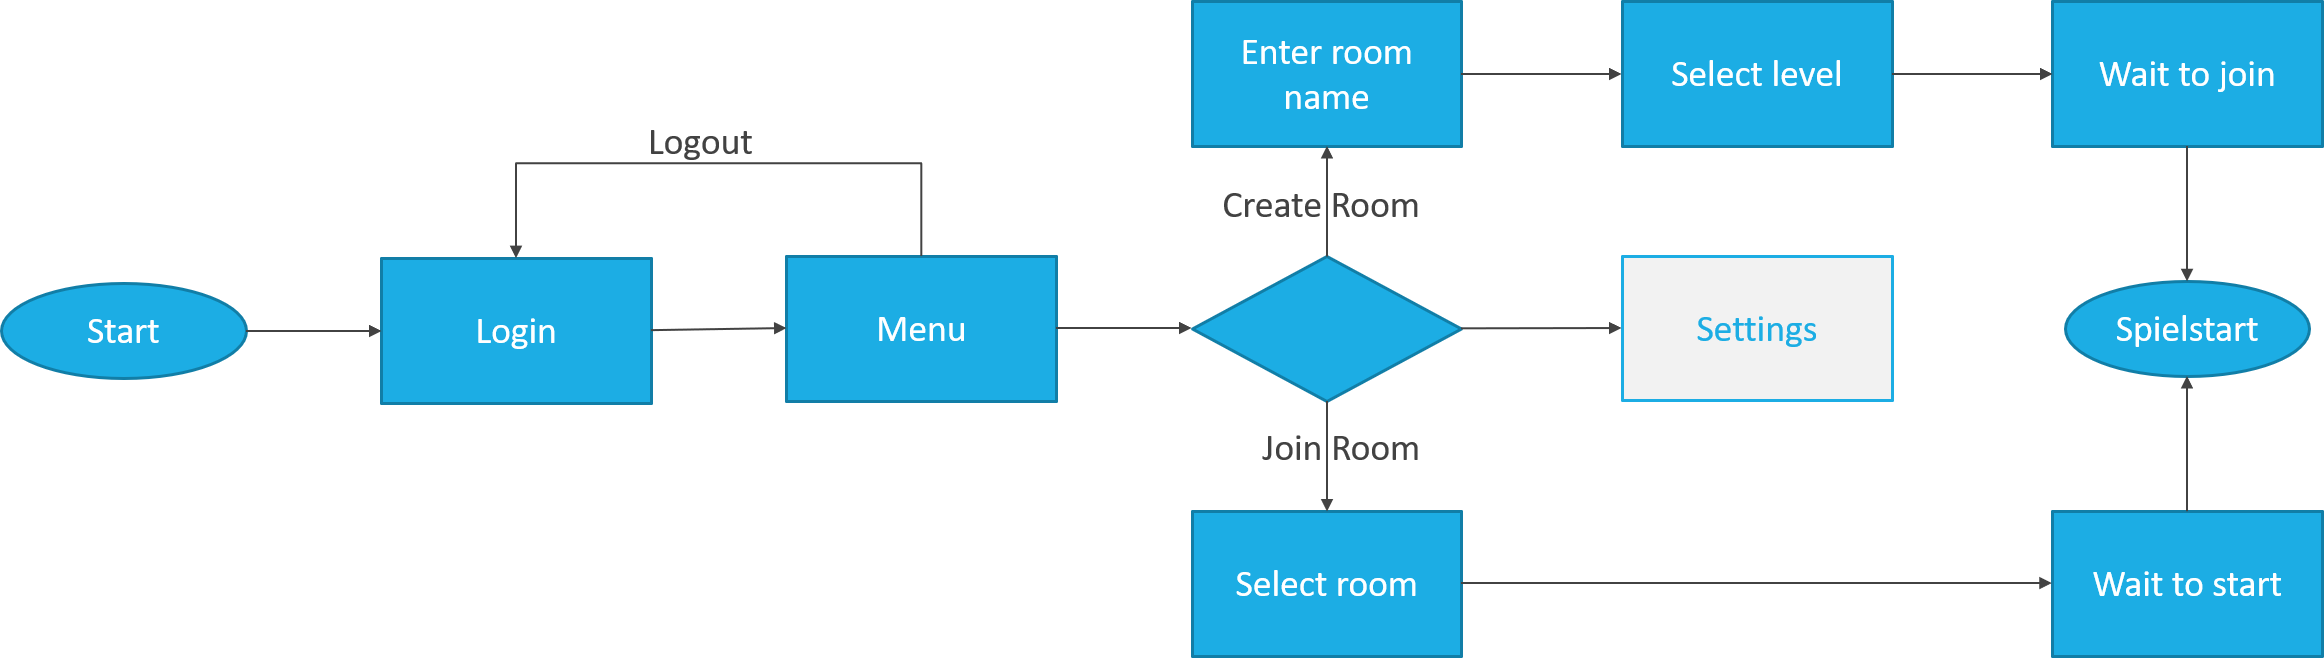
\includegraphics[width=\linewidth]{img/konzeption/Spielablauf2}
      \caption{Menüauswahl}
      \label{fig:konzeption:layout:menu}
    \end{center}
\end{figure}

Neben dem Erstellen bzw. Beitreten eines Raums kann man im Hauptmenü zusätzlich die Musiklautstärke verändern. Dabei kann die Hintergrundmusik, die In-Game-Geräusche und die Klick-Laustärke des Button-Feedbacks eingestellt werden.
\chapter{Implemenentierung}
\label{cha:implementierung}
Kurzes Text

% Abschnitt: Technologien
\section{Technologien}
\label{sec:grundlagen:technologien}

\subsection{Unity}
\label{subsec:grundlagen:technologien:unity}
unity
Vor- und Nachteile
wieso Unity gewählt?
Tiles 
Inspector
Prefabs
usw.

\subsection{Weitere Frameworks}
\label{subsec:implementierung:technologien:frameworks}
Rest
PUN als extra Subsection?
Server als extra Subsection?
Datenbank als extra Subsection?

\subsection{Unity \& Mobile Applications}
\label{subsec:implementierung:technologien:mobile}

\section{Umsetzung}
\label{sec:grundlagen:umsetzung}

\subsection{Nutzerprofile}
\label{subsec:implementierung:umsetzung:nutzerprofile}

\subsection{Multiplayer}
\label{subsec:implementierung:umsetzung:multiplayer}

\subsection{Einstellungen}
\label{subsec:implementierung:umsetzung:einstellungen}

\subsection{Level}
\label{subsec:implementierung:umsetzung:level}

\section{Probleme}
\label{sec:implementierung:probleme}
% Design von Assets -> Kostenlose genommen, da aufwändig

\chapter{Zusammenfassung \& Ausblick}
\label{cha:zusammenfassungAusblick}
In diesem letzten Kapitel wird die Arbeit nochmal zusammengefasst um anschließend einen Ausblick für die Zukunft zu geben.

% Abschnitt: Zusammenfassung
\section{Zusammenfassung}
\label{sec:grundlagen:zusammenfassung}
Da Unity als Engine schon viele vordefinierte Funktionen anbietet, darunter zum Beispiel die Collision Detection, ist das Arbeiten zunächst ungewohnt im Gegensatz zur Arbeit mit einer Entwicklungsumgebung wie Android Studio. Ein Grund dafür ist, das ein großer Anteil nicht über Programmcode, sondern über die GUI Oberfläche die Unity zur Verfügung stellt realisiert wird. Der Inspector des Editors lässt die Componenten der Gameobjects mit den jeweiligen Attributen schnell verändern. Dadurch ist das fertige Spiel sehr wandlungsfähig und kann nach belieben im Detail angepasst werden. 

Nach dem Fertigstellen der App kann durch die gute Kompatibilität von Unity mit sehr vielen Plattformen das Spiel nicht nur auf Android, sondern auf weiteren Plattformen verwendet werden. Dadurch, und durch die Verwendung von Phton, wird unsere Abyss-Anwendung zu einem \textit{Crossplatform game}.

Das Verwenden von eigenen UI-Elementen sollte man als Design-Anfänger oursourcen, da das Erstellen von Bilder, die visuell ansprechend sein sollen, eine künsterische Ader erfordert. Das gleiche gilt für die Erstellung von eigenen Soundeffekten und Hintergrundmusik. Man kann durch die Verwendung von eigenen Materialien das Spiel sehr individualisieren, doch ist der Aufwand, der hinter dieser Arbeit steckt, nicht zu unterschätzen. 

Das Projektmanagement der Unity-Anwendung ist mit Git fehleranfällig. Erstellt man jedoch für jedes Problem einen eigenen Branch können die enstehenden Probleme minimal gehalten werden.

% Abschnitt: Ausblick
\section{Ausblick}
\label{sec:grundlagen:ausblick}
Nachdem das Grundgerüst des Spiels mit den selbstentworfenen Funktionen und Assets erstellt wurde, ist das Spiel schnell und simpel erweiterbar. Durch das Verwenden von Prefabs und den vorhandenen Tilemaps können in kürze Spielflächen erstellt und Hindernisse hinzugefügt werden. Um neue Spielobjekte zu erstellen, können die vorhandenen Skripte angefügt und durch neue, aber simple Skripte erweitert werden. Dadurch kann das Spiel nicht nur an Leveln, sondern auch an Spielkomplexität wachsen.

% Bibliograhpy
\bibliographystyle{splncs}
\begingroup
\interlinepenalty 10000
\sloppy
\bibliography{literature}
\endgroup

% anhänge
\appendix
% hier kommen die anhänge
\chapter{Quelltexte}

In diesem Anhang sind einige wichtige Quelltexte aufgeführt.

\begin{lstlisting}[caption={Zeilencode}]
public class Hello {
    public static void main(String[] args) {
        System.out.println("Hello World");
    }
}
\end{lstlisting}


\backmatter			% abtrennung für verzeichnisse

% hier die verzeichnisse
\listoffigures

\end{document}
